\newpage
\section{Signal Start Detection}
\label{sec:04_signalStartDetection}

\todo[inline]{This section seems a bit misplaced. I feel like "Team Evaluation"
should be the last evaluation section. Is there a reason why you can't put this
before that?}

\todo[inline]{Zwei mal previously}
Previously, the importance of the signal start was underlined
by the results of the previous chapters.
% Due to the fact that the direction detection methods is
% executed on smaller frames than the actual whistle detection.
% To demonstrate this for the phase method, the frame to investigate is
% shifted with time \cref{subsec:04_frameNumber}.
Especially the result in \cref{subsec:03_phase} has shown that in fact, the accuracy
decreases with belated frame.
Also according to the outcome of \cref{subsec:04_psnr}, the \ac{GCC}
method performs best with frames near to the signal start. \todo[inline]{Get
rid of some cross-references and/or write more about what happened in these
chapters. (I don't remember what happened in 3.4 and 4.2.3 and jumping back and
forth is annoying.)}

% There are some reasons why other methods were tested to find the signal start.
In order to find a good solution for a highly reliable, accurate but
computationally reasonable start detection, different approaches were
tested profoundly.
For high accuracy either the number of samples in a frame have to be
small or the window must be shifted with small steps which both implicit
a high number of executions.
The existent whistle detection algorithm of \cref{subsec:03_whistleDetection}
is computationally intensive and causes causes some false positives
for small frames as shown in \label{subsec:04_whistleDetection}.
Therefore, it is looked for more simple algorithms that are not restricted
to whistle sounds only.

Hereinafter, the characteristics of the methods are pointed out by
analyzing the error between algorithmically determined start index
and manually defined start index.
For evaluation, the 11 measurements of on all robots \cref{subsec:04_labMeasurements}
are taken into consideration.
By the frame size of the \ac{FFT} being set to 256 samples for the
correlation methods, a start index error of maximal 256 samples
desired.
Therefore, a start index detection result is regarded as failure for errors
larger than 256 for the following sections.
Two metrics are specified to express the degree of failure.
One counts the number of large errors for each channel.
In this case, 220 sample data for 11 measurements on five robots with
four channels each exist.
Another option is to count if any of the channels failed.
For this case, 55 measurements are given.
% -----------------------------------------------------------------------------------------------------

\subsection{Whistle Detection}
\label{subsec:04_whistleDetection}

First, the accuracy of the whistle detection in regard of the start index
is evaluated.
Here, the start index is defined as the first index where the whistle detection
found a whistle.
With a frame size of 1024, the whistle detection algorithm fails in every of the
55 measurements with at least one channel if only a error of maximal 256 samples
is permitted.
However, every error is in the range of 1024 samples which proves that the
approximate start of the whistle sound is detected correctly.
With a smaller frame size of 256, the error samples decrease but introduces
false positive detections.
With the results, one can say that the whistle detection is not sufficient
for the start detection or is at least not reliable as stand-alone solution.
Furthermore, this approach as it is is limited to sounds in fixed and known frequency range.
%  failure rate of
% 9\si{\percent} in regard to every channel.
% In this work microphone data were saved as soon as the whistle detection module
% found a whistle sound in the audio samples.
% Due to this implementation, the algorithm does never fail to detect the whistle
% Standing alone, the error is always in the range of \si{\pm1024} samples due to the
% set frame size of 1024 samples.
% With a smaller frame size of 256, the accuracy gets better with an error of
% 9\si{\percent} in regard to the 220 sample data but has an error rate of
% 25,5\si{\percent} for the measurements.

% looking at the next 300
% values and with a step size of 50 the result is 15\si{\percent} and 36\si{\percent}
% and with step size 1, it is 13\si{\percent} and 33\si{\percent}.
% This is computationally very costly and the reward is small.

\subsection{ZCR}
\label{subsec:04_zcr}

For the evaluation of the \ac{ZCR},
the frame size is set to 256 samples and number of noise and signal frames
are set to 10 frames.
In 7\si{\percent} of the 220 channel sample data, the method fails with a significant
error larger than 256 samples.
In most cases, the method provides accurate results with small error.
Taking all measurements of robot 26 as example, the \ac{RMSE} amounts
54,23 samples.

However, there are cases where the algorithm fails.
Looking at those cases it could be identified that
the errors occur often due to incorrect assumptions that
the signal is represented at the end of the buffered
samples.
Some measurements prove, that this is not always the case as \cref{fig:04_zcrFail} shows.
Here, the data of the front right channel of robot 21 with the whistle source
at position 5 in \cref{subsec:04_labMeasurements}
illustrates how the signal ended around 35000 samples already.
% -------------------------------------------------------------
\begin{figure}[ht]
	\centering
	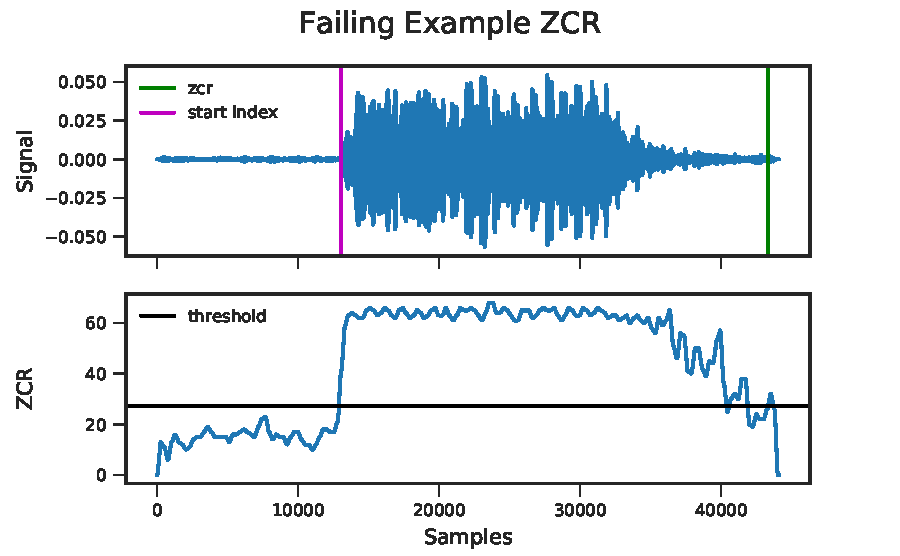
\includegraphics[]{figures/evaluation/zcr_fail}
	\caption{Channel 3 data from measurement 5 of \cref{subsec:04_labMeasurements}
		for robot number 21. A failing example for the start detection by \ac{ZCR}
		is shown.}
	\label{fig:04_zcrFail}
\end{figure}
% -------------------------------------------------------------
If the start index is determined at the point where the \ac{ZCR}
falls below the threshold searching backwards as stated in \cref{sec:02_signalStartDetection},
the detection fails.

In most cases, only one channel of four output a erroneous result.
Because the final start index on one robot is set equal for all channel,
the failure can be compensated with a smart voting procedure.

Another option exists by changing the process of finding the
threshold excess onwards.
In this case, the threshold is raised with a factor of 1,25.
Results by this were poorer than the initially implemented manner
with 15\si{\percent} failure rate.
By adding the constraint that multiple samples must exceed the
threshold successively, result can be slightly improved but implies higher
computational effort.

Worth mentioning is the poor output of the \ac{ZCR} method with
signal that was cleaned with spectral subtraction previously.
This surprising outcome is convenient for the overall task,
because the start index result can be embed into the spectral
subtraction, providing information for separating the noise
and signal part.

\subsection{Entropy}
\label{subsec:04_entropy}

As discussed in \cref{subsec:02_Entropy} the entropy quantifies the amount
of chaos in a signal frame.
Especially for signals to localize with unknown characteristics,
this method can be useful because no a priori knowledge is needed.
For all measurements this method yield poorer results than the \ac{ZCR} method
with a failure rate of around 20\si{\percent}.
Best results are achieved with a frame size of 512 samples and a difference
step of 800 samples.
% \change[]{Explain what steps are? Maybe in implementation?}
However, for records with fading whistle the entropy method
generates more reliable results than the \ac{ZCR} method.
Taking the same measurement as an example where the \ac{ZCR} failed,
\cref{fig:04_entropyGood} shows how the algorithm detects the
signal start correctly even though
the whistle sound ended at around 35000 samples.
In this measurement, the start index errors of all four channels
were smaller than 40 samples.
% -------------------------------------------------------------
\begin{figure}[ht]
	\centering
	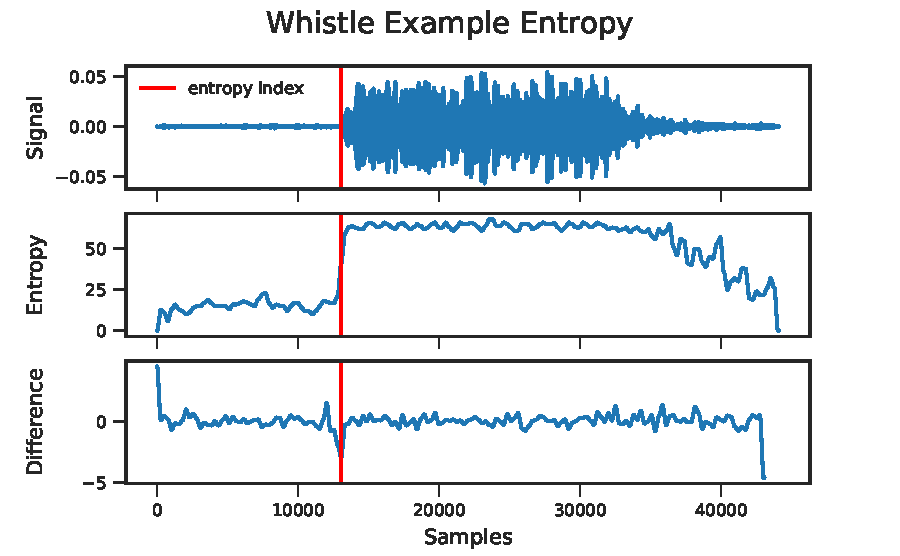
\includegraphics[]{figures/evaluation/entropy_good}
	\caption{Exemplary result of start index detection by entropy where
			the \ac{ZCR} method failed due to fading whistle
			at the data.}
	\label{fig:04_entropyGood}
\end{figure}
% -------------------------------------------------------------

% But as the entropy should be larger for noisy environment
% performance in other surrounding of measurement at \ac{RoboCup} is looked at.
% Entropy would be best for undefined signal -> distinguish between
% signal and noise without information
